% !TeX root = ../main.tex
% -*- coding: utf-8 -*-

\chapter{基于相关统计量的缺陷定位}
本章的研究内容主要针对一种重要的纠错性软件维护手段--缺陷定位。本章首先描述了缺陷定位对维护软件正确性
的作用,然后描述了基于程序谱的缺陷定位方法的一般过程。针对程序中可能存在多错误的问题,本文提出了基于
相关统计量的可疑度计算方法,在计算过程中尽可能避免多错误之间的相互影响。接着阐述了实验评估部分,描述
了实验设置,包括实验对象、对比实验和评价指标。在展示了实验结果和分析之后,对本章进行小结。

\section{引言}
软件系统在当今社会的军事、生活、教育等各个方面占据着重要的地位。随着人们对软件系统依赖性的不断增强,
软件系统失效往往给生活和经济带来巨大的损失,尤其在军事、航空等对可靠性有高要求的行业。软件缺陷是导致
软件失效的主要因素。软件缺陷的存在可能导致软件系统不能按照预期执行,从而造成误差甚至系统崩溃。为了保
证软件正确性,需要软件维护人员及时清除可能导致软件失效的缺陷。

当软件系统失效时,需要对软件系统进行纠错性软件维护,将潜在的软件缺陷清除。缺陷定位指的是当软件失效
时,查找并定位软件缺陷的过程,是纠错性软件维护的基础。虽然缺陷定位是纠错性软件维护的首要条件,但是人
工进行缺陷定位往往是一个冗长而繁复的过程。一方面人工缺陷定位通常依赖软件维护人员的经验和对软件系统的了解,
即使经验丰富的软件维护人员也很难迅速定位导致软件系统行为失效的根本原因。另一方面,针对大规模软件系统,人工缺陷定位所消耗的时间较长,软件维护人员需要充分理解源代码后逐步排查。

为了帮助软件维护人员查找缺陷,研究者们在自动缺陷定位的研究上投入了大量的工作。当前主要的缺陷定位方法
包括基于覆盖分析的方法、基于程序切片的方法、基于程序不变量的方法、基于模型检验的方法、基于状态变更的
方法等。其中大多数方法通过对软件系统的源代码或行为进行建模,查找与软件系统失效的代码。根据建模对象的
不同,传统的缺陷定位方法可以分为动态分析和静态分析两类。前者通过动态分析程序的行为,如执行路径或状态
等,查找相关代码;后者主要通过静态分析软件系统的源代码,从而分析与软件系统失效行为有关的程序元素。虽
然自动化缺陷定位的理论和技术得到了很大的发展,但当前的自动缺陷定位仍然面临两个挑战:

\begin{itemize}
      \item 随着需求的不断增加,软件系统越来越大,导致缺陷定位的效率降低。因此,适用于大规模软件系统的
   的缺陷定位越来越得到关注。
      \item 软件系统中潜在的缺陷可能不止一个,多个软件缺陷之间的相互影响可能导致自动缺陷定位的难度提
      高,准确度下降。尽管目前已经存在部分针对多缺陷的调试技术,但多缺陷的自动定位仍然是不小的挑战。
\end{itemize}

基于覆盖分析的缺陷定位方法,其核心思想是被失效用例执行越多、成功用例执行越少的代码可疑度越高。该类方
法通常只需要统计测试用例的执行结果和覆盖信息,并根据特定的公式计算代码的可疑度,不需要对软件系统的源
代码进行建模,因此计算复杂度低,在面对大规模软件系统时效率较高。然而,引起测试用例失效的软件缺陷可能
不止一个,忽略不同软件缺陷之间的相互影响,可能导致缺陷定位的准确性降低。其主要原因有两个方面:(1)
未被失效用例覆盖的代码可能也包含缺陷;(2)不同软件缺陷共同路径上的正确代码被失效用例覆盖的频率较
大,导致可疑度偏高。本文引入相关统计量的概念,通过将测试用例执行的分支覆盖信息作为特征,测试用例执行结果
作为标签,将原问题转化为数据挖掘问题,从而推测分支覆盖特征对执行结果的重要性。

本章具有以下贡献:

(1)本章提出了基于相关统计量的缺陷定位方法,从数据的角度分析测试用例的覆盖信息,利用特征选择中特征
对分类结果重要性的概念,选择对测试用例执行结果影响较大的分支。

(2)该方法在传统的基于覆盖分析的缺陷定位方法上引入了相关统计量,同样不需要对源代码进行建模,计算复
杂度较低。

(3)针对多缺陷之间相互影响的问题,相关统计量为每个测试用例选择距离最近的同类和异类样本,计算测试用
例在每个分支覆盖特征上距离同类和异类的距离,从而计算分支覆盖特征对测试执行结果的重要性。该方法在很大
程度上避免了多缺陷之间的相互影响。

(4)在开源软件系统上的实验证明,本章方法相比较传统启发式的基于覆盖分析的缺陷定位方法在准确性上具有
一定的提升,通过提高缺陷查找效率缩短了纠错性维护的时间和人力成本。


\section{研究动机与相关工作}
传统的基于覆盖分析的缺陷定位方法,基于启发式的思想使用特定公式计算程序元素的可疑度,其优点在于计算复
杂度低,面对大规模软件系统的效率较高,但也存在一定的问题:由于基于覆盖分析的方法不对程序源代码进行建
模,而是从统计的角度根据代码被失效和成功覆盖的频率推测代码的可疑度,因此对于存在多缺陷的程序,难
以区分不同缺陷导致的失效用例,而缺陷之间的相互影响是导致多缺陷定位的准确性下降的主要原因。

\subsection{研究动机}
\begin{figure}[htp]
      \centering
      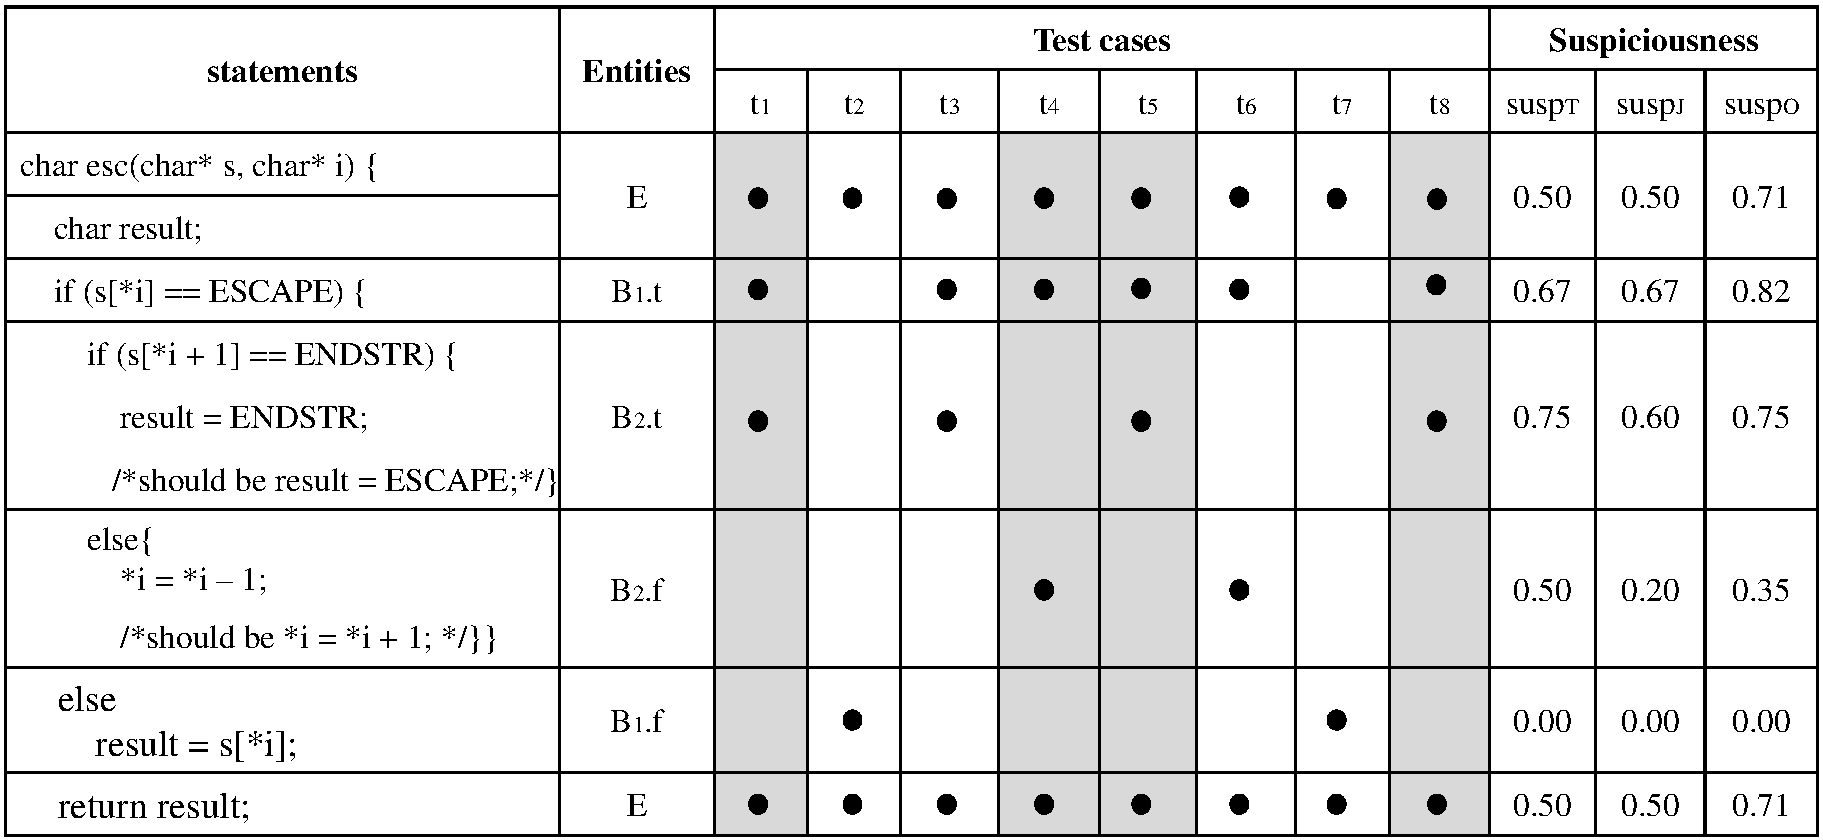
\includegraphics[width=0.95\linewidth]{spectra.pdf}
      \caption{示例程序的分支覆盖特征谱}
      \label{fig:spectra}
\end{figure}

图~\ref{fig:spectra}是示例程序的分支覆盖特征谱,示例代码来自于西门子标准集
\footnote{http://sir.unl.edu/portal/index.php}。图~\ref{fig:spectra}中的示例代码共有2个嵌套的分支结
构,分别是$B_1$和$B_2$。对于每个分支结构,我们用分别用$t$和$f$来示意其两个分支,如$B_1.t$表示第一个
分支结构的真分支。根据分支情况将示例代码分为五个部分,可表示为$P = \{E, B_1.t, B_1.f, B_2.t,
B_2.f\}$,其中$E$表示程序的入口代码快。图~\ref{fig:spectra}中共有8个测试用例,每个测试用例的覆盖信息
表示为一列,黑色圆圈表示该测试用例覆盖了所对应的程序元素。灰色阴影的测试用例表示该用例的执行结果为失
效;反之则为成功用例。右边三列表示用三种经典的可疑度计算公式计算出的可疑度,分别是
Tarantula~\cite{jones2005empirical}、Jaccard~\cite{abreu2007accuracy}和
Ochiai~\cite{abreu2007accuracy}。

以图~\ref{fig:spectra}中的示例代码为例,该代码片段中存在两个缺陷$d_1$和$d_2$,分别在分支结构$B_2$的
真假分支$B_2.t$和$B_2.f$上。失效用例集为$T_f=\{t_1, t_4, t_5, t_8\}$,其中测试用例$t_1, t_5, t_8$覆
盖$d_1$,用例$t_4$覆盖$d_2$。由图~\ref{fig:spectra}可以看出,由于示例代码存在两个缺陷,导致对于每个
缺陷,都存在不覆盖该缺陷的失效用例。例如对于缺陷$d_2$,虽然被失效用例$t_4$覆盖,但是由于缺陷$d_1$的
存在,导致大多数失效用例都不需要覆盖缺陷$d_2$,因此按可疑度比实际偏低。图~\ref{fig:spectra}中的三个
可疑度计算结果可以看到,分支$B_2.f$的可疑度远远比$B_2.t$低,甚至比$E$的可疑度更低。值得注意的是,由
于分支$B_1.t$存在于两个缺陷的共同路径上,因此其被所有的失效用例覆盖,导致其可疑度比实际偏高。

为了说明缺陷个数和基于覆盖分析的可疑度计算之间的关系,本文用$\alpha$表示其被失效用例覆盖的次数占失效
用例总数的比例。当程序中只存在一个缺陷$d$时,所有失效用例均覆盖该缺陷,因此不存在未覆盖该缺陷却导致
测试用例失效的情况,$\alpha=1$永远成立;而当程序中存在不止一个缺陷时,导致测试用例失效的缺陷可能不止
一个,覆盖其中一个或多个缺陷的测试用例都有可能会触发缺陷,导致软件行为失效,因此可能存在失效用例只覆
盖其中部分缺陷,此时$\alpha<=1$;随着具有破坏程序行为能力的缺陷个数越来越多,每个缺陷所触发的失效用
例占失效用例总数比例越来越小,此时$\alpha$也随之变小。

以Tarantula\cite{jones2005empirical}为例,使用$\alpha$可将公式~\ref{eq:tar}表示为:
\begin{eqnarray}
 susp_T = \frac{1}{1+\frac{|T_p|}{\alpha}}, \label{eq:t}
\end{eqnarray}
其中$|T_p|$表示成功用例的个数。从公式~\ref{eq:t}中可以看出,随着软件中包含的缺陷越来越多,由于每个缺
陷所导致的失效用例占总失效用例的比例下降,导致包含缺陷的程序元素所对应的$\alpha$变小,因此缺陷的可疑
度$susp_T$降低,从而影响了缺陷定位的准确度和效率。

\subsection{多缺陷定位相关工作}
在早期研究中,有研究者提出``One-bug-at-a-time''~\cite{klahr1988cognitive},将多缺陷程序视为单缺陷程
序进行定位,在修复缺陷后若还存在失效用例,则继续缺陷定位并修复。这种方法由于忽略了缺陷之间的相互影
响,导致定位缺陷的准确率较低,且由于需要重复执行测试用例集,因此效率较低。

一种理想的解决方式是将由不同缺陷导致的失效用例划分成为不同的失效用例集,对其中每个失效用例集可视为当
前程序只存在一个可触发程序失效的缺陷,其余缺陷均不能引起程序行为失效。在这种情况下,所有失效用例均覆
盖包含缺陷的代码,此时缺陷代码的$a_{01}=0$,因此$\alpha$取得最大值。根据公式~\ref{eq:t}可知,当
$\alpha$取最大值时,缺陷代码的可疑度最高。这种方法的优点在于每个失效用例集均来自于同一缺陷,因此测试用例的直观性比较强,使用单缺陷定位方法能够快速定位到缺陷。

为了达到这个效果,部分学者使用聚类分析将失效用例进行聚类~\cite{jones2007debugging,
zheng2006statistical},对每类失效用例采用单缺陷的方法进行处理。基于聚类分析的方法,其核心思想是由相
同缺陷引起的失效用例其程序行为相似,具有相似的覆盖信息。这种方法虽然在一定程度上提高了多缺陷的定位准
确率,但是依赖聚类分析的准确性,很难完全避免多缺陷之间的相互影响。

文万志等人~\cite{conslice2013}提出使用条件切片进行多缺陷定位,该方法根据输入条件的不同计算出不同的条
件切片,将失效用例进行划分,每类失效用例被视为由同一缺陷引发,最后通过基于覆盖分析的缺陷定位技术计算
可疑度。该方法与基于聚类分析的方法类似,其最终目的是将多缺陷程序当做单缺陷程序处理,在依赖划分准确性
的同时忽略了缺陷之间的相互影响;与之不同的是,本文方法不需要对失效用例进行划分,且不需要进行条件切
片。

基于失效用例划分的多缺陷定位方法~\cite{zheng2006statistical, jones2007debugging, conslice2013}虽然在
一定程度上提高了多缺陷定位的效率,但其准确度依赖于失效用例划分的质量。不准确的划分使得同一失效用例集
中包含来自多个缺陷的失效用例,因此容易导致混入由其它缺陷导致的失效用例,从而引入噪音;除此以外,由于
划分导致每个失效用例集的规模变小,因此可能引起缺陷定位的不准确性。

何加浪等人~\cite{neural2013}提出使用神经网络定位多缺陷,该方法通过学习输入和缺陷之间的关系,计算代码
的各个位置与每个缺陷之间的相关性来定位缺陷。该方法利用神经网络的泛化能力学习代码和缺陷的相关性,需要
提前假定程序中的缺陷个数。而在实际应用中,软件维护人员很难提前知道潜在的缺陷个数。与之不同的是,本文
方法对缺陷个数不敏感,无需假定程序中存在的缺陷个数,且计算复杂度较低,更适用于大规模软件系统。

与本文方法相近的方法是最近邻法~\cite{renieres2003fault},该方法通过对每个失效用例找出与其最相似的成
功用例,并计算两者之间的不同来推测用例失效的原因。与之不同的是,本文受数据挖掘领域的特征选择所启发,
借鉴相关统计量的概念,将缺陷代码视为对测试用例执行结果影响较大的分支覆盖特征,提出了缺陷相关统计量,使被执行
后越容易导致用例失效的代码可疑度越高。

\section{基于相关统计量的缺陷定位算法}
本章在基于覆盖分析的缺陷定位技术的基础引入了相关统计量的概念,从数据挖掘的角度计算代码对程序执行结
果的重要性,通过为每个测试用例寻找距离最近的测试用例,在很大程度上避免了多缺陷相互之间的影响,提升了
缺陷定位的效率和准确率。

\subsection{基于覆盖分析的缺陷定位}
\begin{figure}[htp]
      \centering
      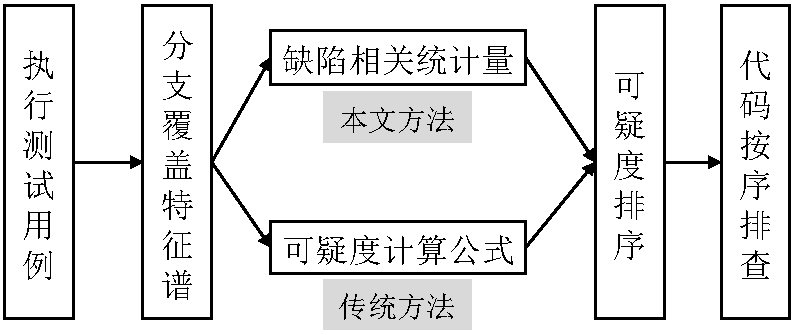
\includegraphics[width=0.6\linewidth]{fault_flow.pdf}
      \caption{覆盖分析法的基本流程}
      \label{fig:fault_flow}
\end{figure}

如图~\ref{fig:fault_flow}所示,基于覆盖分析的缺陷定位技术(以分支覆盖特征为例)主要包括以下三步:

(1)运行测试用例,收集测试用例运行过程中的覆盖信息,得到分支覆盖特征谱;

(2)按照特定的可疑度计算公式为由分支划分的每个代码基本块计算可疑度;

(3)按照可疑度由高至低的顺序对程序源代码进行排查。 

\begin{Definition}
      程序。程序$P$由代码表示,记作$P=\{e_1, e_2, e_3, ..., e_n\}$,其中$e$表示特定的
      程序元素。
\end{Definition}

为了收集测试用例执行的覆盖信息,首先将程序表示为由程序元素组成的序列。常用的程序元素有语句、分支、谓
词、定义对等。根据元素的粒度不同,可以将程序元素分为语句和基本块两类,前者将程序的所有语句表示成一个
序列,记录每条语句的覆盖信息;后者将程序表示为基本块序列,每个基本块由部分程序语句组成(如分支等)。
程序元素可以是基于控制流的程序语句组合(如语句、分支等),也可以是通过数据流分析提取的变量的定义-使
用对,通过关注在成功和失效用例中变量的使用情况来定位缺陷,还可以是其它与程序行为相关的关键代码,如谓
词等。程序元素的多样性使得基于覆盖分析的缺陷定位技术更加灵活和高效。

\begin{Definition}
      软件缺陷。软件缺陷是程序中存在的对程序行为具有破坏能力的错误或功能缺陷,记作$d$。
\end{Definition}

\begin{Definition}
      成功用例。执行测试用例,当且仅当程序$P$的输出与预期输出一致时,称该测试用例为成功用例,成功用
      例集记作$T_t$。
\end{Definition}

\begin{Definition}
      失效用例。执行测试用例,当程序$P$的输出与预期输出不一致时,称该测试用例为失效用例,失效用例集
      记作$T_f$。
\end{Definition}

软件缺陷是导致程序行为与预期不同的主要原因,纠错性软件维护通过查找和修复软件缺陷,提高软件系统的可靠
性。根据测试用例执行的结果是否与预期一致,可以将测试用例集划分为成功用例和失效用例两类。成功执行的测
试用例可能未覆盖软件缺陷,也可能覆盖但并未出发软件缺陷;相反,失效执行的测试用例覆盖并触发至少一个软
件缺陷,导致程序的正常行为被破坏,与预期不一致。

\begin{Definition}
      程序谱。给定程序$P$和测试用例集$T$,程序谱用来记录测试用例集$T$对程序$P$在执行过程中的覆盖信
      息,记作二维矩阵$S_{m\times n}$,其中$m$表示测试用例集的规模,$n$为程序中所含程序元素的个数。
      矩阵元素$S_{ij}$为
      \begin{eqnarray}
         S_{ij} = \begin{cases} 1, & \mbox{第}i\mbox{个测试用例覆盖了第}j\mbox{个程序元素} \\ 
  0, & \text{ 其它 }  
  \end{cases}   , 1 \leqslant i \geqslant  m, 1 \leqslant j \geqslant n
      \end{eqnarray}
\end{Definition}

在确定程序元素后,通过插桩技术记录测试用例执行过程中是否覆盖特定的程序元素,并将结果记录在程序谱
中。需要注意的是,程序谱只记录程序元素的是否被测试用例覆盖,并不记录测试用例执行的顺序,因此程序谱通
常是二维0-1矩阵,其所占内存与测试用例集的规模和程序规模有关,通常在可接受范围内。

\begin{Definition}
     可疑度。程序$P$中的语句或基本块$e$包含缺陷的可能性为其可疑度,记作$suspiciousness(e)$。
\end{Definition}

经典的可疑度计算方法有Tarantula~\cite{jones2005empirical}、Jaccard~\cite{abreu2007accuracy}和
Ochiai~\cite{abreu2007accuracy},其计算公式如下:
\begin{eqnarray}
 susp_T = \frac{\frac{a_{11}}{a_{11}+a_{01}}}{\frac{a_{11}}{a_{11}+a_{01}}+\frac{a_{10}}{a_{10}+a_{00}}}, \label{eq:tar}\\
susp_J = \frac{a_{11}}{a_{11}+a_{01}+a_{10}}, \label{eq:jac}\\
susp_O = \frac{a_{11}}{\sqrt{(a_{11}+a_{01})\times(a_{11}+a_{10})}}, \label{eq:och}
\end{eqnarray}

上述公式中的四个变量均用来描述程序元素覆盖与否信息与执行结果之间的关系:
\begin{itemize}
  \item $a_{00}$表示测试用例被成功执行但未覆盖某个程序元素;
  \item $a_{01}$表示测试用例执行失效且未覆盖某个程序元素;
  \item $a_{10}$表示测试用例被成功执行且覆盖某个程序元素;
  \item $a_{11}$表示测试用例执行失效且覆盖了某个程序元素。
\end{itemize}

基于覆盖分析的缺陷定位方法,除部分结合切片技术的方法~\cite{conslice2013,wen2013}外,其大致流程通常不
变,通过改变可疑度计算公式来提高方法的准确率和效率。缺陷定位的目的是查找引起程序行为失效的程序代码。
不考虑外部因素,失效用例的执行路径至少覆盖一个软件缺陷,且不覆盖软件缺陷的测试用例一定是成功用例。因
此,是否覆盖缺陷代码与测试用例否失效之间存在一定的相关性。本文假设是否覆盖缺陷代码是判断程序行为是否
失效的重要因素,借鉴特征选择中的相关统计量概念计算代码对程序行为结果的重要性,从而定位软件缺陷。如图
~\ref{fig:fault_flow}所示,在基于覆盖分析的缺陷定位基础上,受特征选择启发,引入了相关统计量的概念,
并提出了缺陷相关统计量来计算代码的可疑度,提高了定位缺陷的额准确率和效率。

\subsection{Relief特征选择模型}
现实问题中往往存在大量的特征,然而不是所有特征都与任务目标有关。根据与任务目标的相关性,可以将特征分
为无关特征和相关特征两类。与任务目标毫无关联的特征一般被称为``无关特征'',大量的无关特征可能会导致特
征的维度过高,造成``维度灾难'',同时可能导致训练难度的提高。因此,去掉无关特征可以在降低数据维度的同
时降低训练难度,对模型训练是有益的。另一类与任务目标有关的特征通常被称为``有关特征'',然而有关特征之
间并一定是相互独立的,可能存在部分特征可以通过其它特征计算得到,这类特征通常记作``冗余特征''。虽然冗
余特征可以通过其它特征获得,但并不代表冗余特征一定是无益的。部分冗余特征通过对其它特征的整合,使得其
本身更接近学习任务,因此可以降低学习的难度。因此,冗余特征不一定要全部移除,根据特征与学习目标的关
系,可将冗余特征分为``有益特征''和``无益特征''。特征选择的目的就是去除特征集合中的与学习任务不相干的
``无关特征'',以及虽然与学习任务相关,但可以由其它特征计算而来且对学习任务没有益处的``冗余特征''。

Relief特征选择模型由Kira~\cite{kira1992feature}等人提出,最早用来针对二分类问题在数据预处理阶段进行
特征选择,从而降低数据维度。Relief特征选择模型的核心思想是通过估算特征对相似样本的区分能力来判断特征
是否对二分类学习任务有益。样本的相似性通过样本之间的距离来衡量,给定距离公式,距离越小的样本,相
似性越大。特征对相似样本的区分能力体现在,对任意一个样本以及与其最相似的同类样本和异类样本,若在某个
特征上,样本总是倾向于与同类样本的距离近,而与异类样本的距离远,则认为该特征上对相似样本具有区分能
力。

为了衡量特征对相似样本的区分能力,Kira~\cite{kira1992feature}等人引入了相关统计量的概念,计算每个特
征与二分类类别之间的相关性,并将其作为特征的权重,提出了一种基于特征权重的算法,通过移除权重低于特定
阈值的特征来进行特征选择。具体来说,给定样本集$\mathcal D=\{(x_1,y_1),(x_2,y_2),...,(x_n,y_n)\}$,和
原始特征集$\mathcal F=\{f_1,f_2,...,f_q\}$,其中$q$为原始特征的个数,
$x_i=\{x_{i1},x_{i2},...,x_{iq}\}$,。从训练样本集$\mathcal D$中随机抽取一个样本$(x_i,y_i)$,Relief
特征选择模型分别为样本$(x_i,y_i)$寻找一个同类样本$(x_{i,nh},y_i)$(记作$near-hit_i$)和一个异类样本
$(x_{i,nm},-y_i)$(记作$near-miss_i$),然后分别计算$x_i$与$x_{i,nh}$和$x_i$与$x_{i,nm}$在第$j$个特
征上的距离之差:
\begin{equation}
       \delta^j_i = -\text{diff}(x_i^j, x_{i,nh}^j)^2 + \text{diff}(x_i^j,x_{i,nm}^j)^2, \label{eq:delta}
\end{equation}
当特征$f_j$为离散型时:
\begin{equation}\label{eq:lisan}
       \text{diff}(x^j_a,x^j_b) = \begin{cases} 0, & \textit{if}~x^j_a=x^j_b \\ 
  1, & \text{ otherwise, }  
  \end{cases} 
\end{equation}
当特征$f_j$为连续型时:
\begin{equation}
       \text{diff}(x^j_a,x^j_b) = |(x^j_a-x^j_b)|.
\end{equation}
重复上述过程,从样本集中随机抽取样本$M$次,得到关于特征$f_j$的相关统计量:
\begin{equation}
       \delta^j = \frac{1}{M}\sum_{i=1}^M{-\text{diff}(x_i^j, x_{i,nh}^j)^2 + \text{diff}(x_i^j,x_{i,nm}^j)^2}. \label{eq:Delta}
\end{equation}

从公式~\eqref{eq:delta}中可以看出,在第$j$个特征上,当$x_i$与其最近同类$x_{i,nh}$距离小,与其最近异
类$x_{i,nm}$距离大时,说明此时该特征对区分不同类别的样本是有益的,因此增加特征$f_j$的权重
$\delta^j_i$;反之,若$x_i$与其最近同类$x_{i,nh}$距离大,而与其最近异类$x_{i,nm}$距离小时,说明此时
该特征对区分不同类别的样本是无益的,此时减小特征$f_j$的权重$\delta^j_i$。

\begin{algorithm}[H]
\caption{Relief特征选择算法}\label{alg:relief}
\KwIn{样本数据集$\mathcal D$,原始特征集$\mathcal F$,相关统计量阈值$\Gamma$,样本抽取次数$M$;}\\
\KwOut{特征子集$\mathcal {V}$,特征的相关统计量$\delta$;} \\
初始化特征子集$\mathcal {V} \leftarrow \emptyset$;\\ 
初始化每个特征的相关统计量$\bm \delta^j \leftarrow \bm 0$;\\ 
根据样本标签将样本数据集$\mathcal D$划分为正类$\mathcal D^+$和负类$\mathcal D^-$;\\
\For {$i=1$ to $|M|$} {
     从样本数据集$\mathcal D$中随机抽取一个样本$(x_i,y_i)$;\\
     从数据集$\mathcal D^+$和$\mathcal D^-$中分别寻找距离$x_i$最近的两个样本,其中与$(x_i,y_i)$同类的样本为$(x_{i,nh},y_i)$,与$(x_i,y_i)$异类的样本为$(x_{i,nm},y_i)$;\\
     \For {$j=1$ to $|\mathcal F|$} {
            根据当前样本$(x_i,y_i)$计算在特征$f_j$的相关统计量$\delta^j_i$(公式~\eqref{eq:delta});\\
            更新特征$f_j$的相关统计量$\delta^j \leftarrow \delta^j + \delta^j_i$;\\
     }
}
\For{$j=1$ to $|\mathcal F|$} {
      计算平均相关统计量$\delta^j \leftarrow \frac{\delta^j}{M}$;\\
      \If{$\delta^j \geqslant \Gamma$}{
            添加特征$f_j$进入特征子集$\mathcal V$;\\
      }
}

\textbf{return} 特征子集$\mathcal {V}$,每个特征的相关统计量$\delta$。\\
\end{algorithm}

算法~\ref{alg:relief}为Relief特征选择模型的算法,Relef为每个测试用例寻找距离最近
的同类和异类样本,距离同类越近、距离异类越远的特征被认为越能够区分不同类别的样
本。从算法~\ref{alg:relief}中可以看出Relief特征选择的运行时间与原始特征集的规模
$|\mathcal F|$和样本的随机抽样次数$M$线性相关,因此该算法的效率较高。

\subsection{缺陷相关统计量}
\textbf{(1)原理与定义}

借鉴特征选择中的相关统计量概念,是否覆盖缺陷代码可以被认为是对相似测试用例的执行
结果有区分能力的重要因素。缺陷定位的目的是查找能够引起程序行为失效的程序代码,因
此对缺陷代码的执行与程序行为失效之间必然存在某种关联性。不考虑外部因素,失效用例
的执行路径中应该覆盖一个或多个软件缺陷,而不覆盖任何缺陷代码的测试用例理论上一定
是成功用例。因此,是否覆盖缺陷代码与测试用例执行是否失效之间存在一定的相关性。本
文假设可以通过测试用例的执行路径来预测测试用例是否失效,因此,将测试用例在执行过
程中对代码的覆盖信息作为输入数据,测试用例的执行结果作为二分类标签,可以构建一个
二分类模型。可以通过估算覆盖特征对相似测试用例是否失效的区分能力,来选择重要的覆
盖特征,从而定位软件缺陷。需要注意的是,本章接下来以分支覆盖特征为例,但实际上本
章提出的缺陷相关统计量可用于其它程序谱,如语句、谓词、定义对等。

给定程序$P$和测试用例集$\mathcal T$,将该测试用例集作为样本数据集$\mathcal D$,
则测试用例集中的一个测试用例$T_i$可视为一个样本$\mathcal D_i=(x_i,y_i)$,其中
$x_i$表示测试用例$T_i$对代码的分支覆盖特征,用
$x_i=\{x_i^1,x_i^2,x_i^3,...,x_i^n\}$来表示,其中$n$为程序中所含分支覆盖特征的个
数,即原始特征的个数。$x_i^j$为:
\begin{equation}\label{eq:cov}
      x_i^j = 
       \begin{cases}
             1, & \mbox{测试用例}T_i\mbox{覆盖第}j\mbox{个程序元素}\\ 
  0, & \mbox{测试用例}T_i\mbox{未覆盖第}j\mbox{个程序元素},  
       \end{cases}
\end{equation}
也是样本的原始特征;$y_i$表示测试用例$T_i$的执行结果(成功或失效),也是样本的标签$y_i$:
\begin{equation}
      y_i = 
       \begin{cases}
             1, & T_i\mbox{是成功用例}\\ 
  -1, & T_i\mbox{是失效用例}.  
       \end{cases}
\end{equation}

\textbf{(2)存在的问题}

结合基于覆盖分析的缺陷定位技术,本文认为缺陷代码的覆盖信息与测试用例执行的结果应该有以下相关性:
\begin{itemize}
      \item 失效用例的执行路径覆盖至少一个缺陷;
      \item 不覆盖缺陷代码的测试用例一定是成功用例;
      \item 被失效用例覆盖越多、成功用例覆盖越少的代码越有可能是缺陷代码。
\end{itemize}

本章在基于覆盖分析的缺陷定位基础上,受特征选择启发,引入了相关统计量的概念来定位
缺陷。相关统计量最早被用来做二分类之前的特征选择,其主要思路是将对相似样本有区分
能力的特征作为重要的特征。当使用相关统计量来进行缺陷定位时,根据公式
~\ref{eq:Delta},特征$f_j$的相关统计量$\delta^j$较高的可能存在以下四种原因:
\begin{itemize}
      \item 当$x_i^j=0$时,$y_i=1$总是成立;
      \item 当$x_i^j=0$时,$y_i=-1$总是成立;
      \item 当$x_i^j=1$时,$y_i=1$总是成立;
      \item 当$x_i^j=1$时,$y_i=-1$总是成立。
\end{itemize}

换句话说,相关统计量所代表的含义仅仅是特征与分类结果的相关性,而与测试用例执行结
果相关的代码并不一定包含缺陷代码,直接使用特征选择的概念来计算相关统计量,容易导
致以下代码的相关统计量偏高:

a. 当测试用例的执行路径未覆盖某个分支时,测试用例总是成功执行;

b. 当测试用例的执行路径未覆盖某个分支时,测试用例总是失效执行;

c. 当测试用例的执行路径覆盖某个分支时,测试用例总是成功执行;

d. 当测试用例的执行路径覆盖某个分支时,测试用例总是失效执行。

根据公式~\ref{eq:Delta},上述四种可能中的代码对测试用例执行结果的区分能力较强,因此相关统计量较高。
然而,这与定位缺陷代码的目的并不完全一致。虽然覆盖缺陷代码与测试用例执行结果是否失效存在一定的关联
性,但是相关统计量高的代码未必可疑度高,因为对测试用例的执行结果有较强区分能力的代码包括但并不完全等
价于覆盖后容易导致测试用例失效执行的代码。具体来说,根据缺陷分支覆盖特征与测试用例执行结果的相关性,
在上面的四种相关统计量较高的可能情况中,只有a和d两种情况暗示着该分支有较大可能是缺陷相关分支,而b和c
两种情况则完全相反,暗示着该分支很有可能是缺陷无关分支。

\textbf{(3)缺陷相关统计量}

Relief算法中的相关统计量只用来衡量特征与二分类结果的相关性,而并未给出特征是如何影响分类结果的。为了
研究相关统计量与代码可疑度之间的关系,本文提出缺陷相关统计量的概念来估算程序代码与缺陷性相关性,,并
以此作为代码的可疑度。首先,由于测试用例的执行路径只有``覆盖''和``不覆盖''某个程序元素两种可能,因此
分支覆盖特征是离散型0-1变量,我们将公式~\ref{eq:lisan}代入公式~\ref{eq:delta}可得相关统计量为:
\begin{equation}
       \delta^j_i = -\llbracket x_i^j \neq x_{i,nh}^j \rrbracket + \llbracket x_i^j \neq x_{i,nm}^j \rrbracket, \label{eq:delta2}
\end{equation}
从公式~\ref{eq:delta2}中可以看出,给定分支$f_j$,随机抽取一个测试用例$x_i$并寻找距离该用例最近的一个
同类用例$x_{i,nh}$(near-hit)和一个异类用例$x_{i,nm}$(near-miss)。只要在分支$f_j$上$x_{i,nh}$与
$x_i$的覆盖情况相同,而$x_{i,nm}$与$x_i$的覆盖情况不相同,则有$\llbracket x_i^j \neq x_{i,nh}^j
\rrbracket=0$,$\llbracket x_i^j \neq x_{i,nm}^j \rrbracket=1$,此时$\delta_i^j=1$,增加分支$f_j$的
相关统计量$\delta^j$。

考虑一种情况,当随机抽取的测试用例$x_i$是失效用例($y_i=-1$)时,若此时$x_i^j=x_{i,nh}^j=0$,且有
$x_{i,nm}=1$,则按照公式~\ref{eq:delta2}可得,此时$\delta_i^j=1$,应该增加相关统计量$\delta^j$。然
而,在这种情况下,失效用例$x_i$和$x_{i,nh}$均未覆盖第$j$个代码块,反而成功用例$x_{i,nm}$覆盖了第$j$
个代码块。根据代码被失效执行越多、成功执行越少则可疑度越高的原理,此时减少覆盖分支$f_j$的可疑度。

由此可以看出,Relief算法中相关统计量的更新只与样本和最近同类、异类样本的距离有关,而缺陷定位中覆盖特
征的可疑度的更新还需要考虑随机抽取的测试用例$x_i$的类别$y_i$(成功或失效)以及其是否覆盖分支$f_j$。本文与传统的覆盖分析法基于类似的思想,即被失效用例覆盖越多、成功用例覆盖越少的代码可疑度越
高。因此,根据随机抽取测试用例的类别和对分支$f_j$的覆盖情况不同,可分为以下四种情况:
\begin{itemize}
      \item 当随机抽取的测试用例为失效用例且未覆盖分支$f_j$时,若此时$\delta_i^j$较大,则说明分支
      $f_j$同样未被相似的失效用例所覆盖,而是被相似的成功用例所覆盖,此时应该减小分支$f_j$的可疑度;
      \item 当随机抽取的测试用例为失效用例且覆盖了分支$f_j$时,若此时$\delta_i^j$较大,则说明分支$f_j$同样被相似的失效用例所覆盖,且未被相似的成功用例所覆盖,此时应该增加分支$f_j$的可疑度;
      \item 当随机抽取的测试用例为成功用例且未覆盖分支$f_j$时,若$\delta_i^j$较大,则说明此时分支$f_j$未被相似的成功用例所覆盖,而是被相似的失效用例所覆盖,因此应该增加分支$f_j$的可疑度;
      \item 当随机抽取的测试用例为成功用例且覆盖了分支$f_j$时,若$\delta_i^j$较大,则说明此时分支$f_j$同样被相似的成功用例所覆盖,且未被相似的失效用例所覆盖,因此应该减小分支$f_j$的可疑度。
\end{itemize}

表~\ref{tbl:list}中总结了在不同的情况下,相关统计量与可疑度的关系:
\begin{center}
\tablecaption{相关统计量与可疑度的关系}\label{tbl:list}
\begin{tabular}{|l|l|l|}
\hline
测试用例 & 是否覆盖分支$f_j$ & 相关统计量$\delta^j$与可疑度$\epsilon^j$的关系\\ \hline
\multirow{2}{*}{失效用例} & 未覆盖 & $\epsilon^j$随着$\delta^j$的增加而减小\\
& 覆盖 & $\epsilon^j$随着$\delta^j$的增加而增加\\ \hline
\multirow{2}{*}{成功用例} & 未覆盖 & $\epsilon^j$随着$\delta^j$的增加而增加\\
& 覆盖 & $\epsilon^j$随着$\delta^j$的增加而减小\\ \hline
\end{tabular}
\end{center}

表~\ref{tbl:list}中的$\epsilon^j$表示分支$f_j$的可疑度。可以看出,随机抽取测试用
例后,对每个分支的可疑度的更新与该测试用例是否成功执行以及是否覆盖该分支有关。根
据表~\ref{tbl:list},本文提出了缺陷相关统计量$\epsilon$来估算可疑度。给定分支
$f_j$,随机抽取测试用例$(x_i,y_i)$后,关于分支$f_j$在测试用例$(x_i,y_i)$上缺陷相
关统计量为:
\begin{equation}
       \epsilon_i^j = -y_ix_i^j(-\llbracket x_i^j \neq x_{i,nh}^j \rrbracket + \llbracket x_i^j \neq x_{i,nm}^j \rrbracket). \label{eq:epsilon}
\end{equation}

最后通过从样本集$\mathcal D$中随机抽取样本M次并重复上述计算过程,可得到关于分支
$f_j$的缺陷相关统计量:
\begin{equation}
       \epsilon^j = \frac{1}{M}\sum_{i=1}^M{ -y_ix_i^j(-\llbracket x_i^j \neq x_{i,nh}^j \rrbracket + \llbracket x_i^j \neq x_{i,nm}^j \rrbracket)}. \label{eq:epsilon2}
\end{equation}

需要注意的是,在随机抽取一个测试用例$(x_i,y_i)$后,按照算法~\ref{alg:relief}的第
8行,需要在成功用例集$\mathcal D^+$和失效用例集$\mathcal D^-$中分别寻找一个举例
该测试用例最近的用例。根据公式~\ref{eq:cov},测试用例的特征$x_i^j$可作为布尔值,
因此本文使用曼哈顿距离来计算测试用例$x_a$和$x_b$之间的距离:
\begin{equation}
      \text{distance}(x_a,x_b) = \sum_{i=1}^n{|x_a^i-x_b^i|}
\end{equation}

\subsection{代码排查方案}
如图~\ref{fig:fault_flow}所示,在获得测试用例集$/mathcal T$对程序$P$执行过程中的
分支覆盖信息后,本文将以测试用例作为样本数据,提出了缺陷相关统计量,利用算法
~\ref{alg:relief}估算分支特征的可疑度(算法~\ref{alg:relief}中的第10行改为缺陷相
关统计量公式~\ref{eq:epsilon}),最后按照可疑度由高至低按需排查相关代码。

给定程序$P$,在执行测试用例集后,收集分支覆盖信息得到如图~\ref{fig:spectra}所示的分支覆盖特征谱,利用
Relief算法~\ref{alg:relief}计算分支特征的相关统计量,并提出缺陷相关统计量的计算方式(公式
~\ref{eq:epsilon2})来代替原有的相关统计量,并将所有分支特征按照缺陷相关统计量由高至低排序,得到分支
覆盖特征序列$\mathcal B=\{B_1,B_2,B_3,...,B_n\}$,最后按照可疑度由高至低进行排查。

算法~\ref{alg:search}为根据分支覆盖特征的可疑度排查代码的算法。以图~\ref{fig:spectra}中的分支$B_2.f$
为例,由于$B_2.f$为分支结构$B_2$的一个分支,因此首先排查其所在分支结构$B_2$的判定语句,即第4行语句;
由于不存在与该判定语句在同一个基本块且可以影响到判定结果的语句,因此直接检查分支$B_2.f$中的可执行语
句(*i=*i-1)。

\begin{algorithm}[H]
\caption{代码排查算法}\label{alg:search}
\KwIn{程序$P$,分支覆盖特征序列$\mathcal B$;}\\
\For {$i=1$ to $|B|$} {
      //对分支覆盖特征$B_i$进行排查 \\
      \If{$B_i$是分支结构的一个分支}{
            排查$B_i$所在分支结构的判定语句$S_j$;\\
            排查与判定语句$S_j$在一个代码基本块内,且可能影响到其判定结果的语句;\\
            排查在$B_i$内且控制依赖于分支$B_i$的语句;\\
      }
      \Else{
            排查与$B_i$同在一个函数的所有必须被执行的可执行语句,包括部分分支结构的判定语句;\\
      }
}
\end{algorithm}

\section{实验设计}
本节评估了基于相关统计量的缺陷定位技术和其它主流的基于覆盖分析的缺陷定位方法的有效性,在开源数据集上
通过对比实验验证了本文方法的有效性。

\subsection{实验对象}

为了评估缺陷定位方法的有效性,选取了来自开源软件仓库~\footnote{http://sir.unl.edu/portal/index.php}
(Software Infrastructure Repository,以下简称SIR)的Siemens程序集和flex程序作为实验对象。表
~\ref{tbl:subjects1}中列出了本次实验中实验对象的相关统计数据。


\begin{center}
\tablecaption{实验对象}\label{tbl:subjects1}
\begin{tabular}{|c|c|c|c|c|}
\hline
实验程序 & 代码行数 & 缺陷版本数 & 测试用例数\\ \hline
print\_tokens & 563 & 3 &4130\\ \hline
print\_tokens2 & 508 & 8 & 4115\\ \hline
replace & 563 & 28 & 5542\\ \hline
schedule & 410 & 6 & 2650\\ \hline
schedule2 & 307 & 4 & 2710\\ \hline
tot\_info & 406 & 20 & 1052\\ \hline
tcas & 173 & 39 & 1608\\ \hline
flex & 12\textasciitilde14k & 51 & 567\\ \hline
\end{tabular}
\end{center}

其中,Siemens程序集经常作为基准程序集用来评估缺陷定位方法的有效性~\cite{guanlian2013,con-prob2018},
包括7个C语言程序,其中print\_tokens和print\_tokens2为词法分析器,replace为一个模式替换程序,schedule
和schedule2为两个优先级调度程序,tot\_info可用来进行信息度量,tcas为ADL解释器。除程序源代码外,SIR提
供了植入缺陷的程序版本以及测试用例集。除了Siemens程序集外,使用flex词法分析器来评估方法的有效性。由
于flex是Unix系统中真实使用的程序,因此除了植入的缺陷外,其中还包含部分真实存在的软件缺陷。从表
~\ref{tbl:subjects1}中可以看出,Siemens程序集中的代码行数在170\textasciitilde565之间,属于小规模程
序,而flex的代码行数在12\textasciitilde14k之间,属于大规模程序。

需要注意的是,表~\ref{tbl:subjects1}中所列的缺陷版本数量为经过筛选后的缺陷版本。跟传统的基于覆盖分析
的缺陷定位研究相似,本文在选择缺陷程序版本的时候,进行以下筛选:(1)排除了无法被现有测试用例集所触
发的缺陷版本,即在现有测试用例在执行该缺陷版本时均为成功用例,无法根据测试用例的执行结果判断此时是否
存在缺陷;(2)排除了由代码缺失引起的缺陷,因为基于覆盖分析的缺陷定位研究通常根据代码的覆盖信息与测
试用例的执行估算代码的可疑度,而缺失的代码既不会有覆盖信息,也不存在相应的可疑度,因此在评估方法有效
性时存在问题;(3)排除了有可能引起程序运行时出现异常(segment fault),导致程序运行突然中止的缺陷,
由于基于覆盖分析的缺陷定位技术依赖于测试用例集在整个程序执行过程中对代码的覆盖信息,而可能出现异常中
止的程序导致部分测试用例的覆盖信息不完全,在计算可疑度的时候与其它测试用例不一,因故在实验中将这部分
缺陷排除。最后在实验中一共使用了108个缺陷,并在实验中通过控制一个程序中所注入缺陷的个数来分别构造单
缺陷和多缺陷的程序。

本章在ubuntu14.10系统下进行实验,使用的gcc编译器版本为4.4.1。在执行测试用例之前,使用开源语法分析工
具antlr(版本为3.5.1)在程序的入口和各个分支处进行插桩。然后,通过脚本执行SIR提供的测试用例集,并用
antlr收集分支覆盖信息,得到分支覆盖特征谱。通过比较测试用例在程序的正确版本和缺陷版本上的执行结果是
否相同,判定测试用例为成功用例或失效用例。

\subsection{评价指标}
缺陷定位技术的目的是帮助软件维护人员尽快找到缺陷相关代码,因此缺陷定位技术的有效性和效率通常体现在如
何通过排查尽可能少的代码,尽快定位到缺陷相关代码。基于覆盖分析的缺陷定位技术,通常根据覆盖特征谱按照
特定计算公式计算代码的可疑度,然后按照可疑度由高至低排查相关代码。因此,为了尽可能排查较少的代码,缺
陷相关代码的可疑度排名通常越高越好。

为了评估方法的有效性,本章使用定准率$\beta$和排查率$P_{search}$两个度量方式来从不同的角度对方法进行
比较。定准率表示定位到缺陷相关语句所不需要检查的代码的比例,可表示为:
\begin{equation}
       \beta = \frac{L-L_s}{L-1},\label{eq:beta}
\end{equation}
其中$L$表示程序中可执行代码的总行数,$L_s$为定位到某个缺陷所需要排查的可执行代码的总行数。从公式
~\ref{eq:beta}中可以看出,给定程序$P$,程序中的可执行代码总数固定后,定位到缺陷所需要排查的行数越
小,定准率越高。从公式~\ref{eq:beta}中可以看出,缺陷定位技术并不一定会提高定位缺陷的效率,当定准率
$\beta$小于一定阈值时,反而会降低定位缺陷的效率。例如,当$\beta$小于缺陷按照代码执行顺序所在的相对位
置比时,利用缺陷定位方法查找缺陷的效率比按照代码执行的顺序逐步排查更低。

代码排查率$P_{search}$表示定位到缺陷所需要排查的代码行数与可执行代码总行数的百分比,可表示为:
\begin{eqnarray}
      P_{search}=\frac{|L_s|}{L}\times100\%
\end{eqnarray}
与定准率相反,当缺陷个数固定时,代码排查率越低表示定位到缺陷所需要排查的可执行代码比例越小,因此缺陷
定位效率越高。

\section{实验结果与分析}
\subsection{单缺陷对比实验}
为了评估本文提出的基于相关统计量的缺陷定位方法的有效性,本文与三个经典的可疑度计算方法进行比较,分别
是Tarantula、Jaccard、与Ochiai。

表~\cite{}为实验的结果

\subsection{多缺陷对比实验}
\subsection{适用性讨论}

多错误分类

本以分支覆盖特征谱为例,提出了基于相关统计量的缺陷定位方法。值得注意的是,本章方法也同样适用于其它
程序元素。
依赖测试用例集的质量。如果特别不平衡的话,还是容易导致某些缺陷被放大,某些缺陷被缩小。
\section{本章小结}
,并提出了缺陷相关统计量来计算
代码的可疑度,提高了定位缺陷的额准确率和效率。虽然基于相关统计量的缺陷定位与聚类分析的方法是基于相似
的核心思想,即由相同缺陷引起的失效用例具有一定的相似性,但本文方法在该思想的基础上加了较大的约束,即
本文认为只有距离失效用例最近的失效用例才可能由同一缺陷引起,因此在很大程度上避免了对聚类分析准确性的
依赖,且不需要聚类分析中的参数设置(如缺陷个数等参数)。

通过为每个测试用例选择距离其最近的同类和异类测试用例,为每个失效用例找到最有可能与其由同一缺陷出发的
失效用例。

对相似测试用例的执行结果有区分能力的代码不一定是缺陷代码,
本章提出在覆盖分析的基础上使用相关统计量来定位缺陷,选择对相似测试用例的执行结果有区分能力的覆盖特征作为可能的缺陷代码。

